\documentclass[10pt,letterpaper]{article}

\usepackage{pslatex}
\usepackage{apacite}
\usepackage{graphicx}
\usepackage{ccn}
\usepackage{amssymb,amsmath,amsthm}
\newtheorem{assumption}{Assumption}

\title{Action Grammars: Grammar Induction-Based Learning of Temporal Abstractions}
 
\author{{\large \bf Robert Tjarko Lange (rtl17@imperial.ac.uk)} \\
  Einstein Center for Neurosciences Berlin, Charitéplatz 1, 10117, Berlin, Germany \AND {\large \bf Aldo Faisal (a.faisal@imperial.ac.uk)} \\
  Imperial College London, South Kensington Campus, London SW7 2AZ, United Kingdom}


\begin{document}

\maketitle


\section{Abstract}
{
\bf
Hierarchical Reinforcement Learning algorithms have been applied to large-scale problems with sparse reward signals. By operating at multiple time scales, the Reinforcement Learning agent is able to overcome difficulties in exploration and value information propagation. Current approaches either require previous (manual) specification of hierarchical structures, lack clear interpretability or can hardly be justified in a comparative fashion.
This work combats all of the shortcomings in a fully automated and end-to-end fashion. By treating an on-policy trajectory as a sentence sampled from the policy-conditioned language of the environment, we are able to apply powerful ideas from computational linguistics to the sub-structure discovery problem.
We identify hierarchical constituents with the help of unsupervised grammatical inference. The resulting set of temporal abstractions is called \textit{action grammar} and can efficiently be deployed in multiple challenging Reinforcement Learning settings.
}
\begin{quote}
\small
\textbf{Keywords:} 
Decision Making; Reinforcement Learning; Computational Linguistics
\end{quote}

\section{Introduction}

Human infants learn seemingly unstructured patterns in nature and from observing role models. They are incredibly well equipped to infer hierarchical rule-based structures from language, visual input as as well as auditory stimuli \cite{Frank_2009, Marcus_2007}. By observing an expert, they get a head-start in their learning process and are able to learn over higher level sequences of low level control elements. Furthermore, there is convincing evidence from several MEG and fMRI studies that indicates a universal form of hierarchical language comprehension in the brain \cite{Frank_2018, Brennan_2016, Nelson_2017} and a parallelism to motor control \cite{Pastra_2012, Stout_2018}.
Inspired by such observations, this work overcomes the identified weaknesses by merging Hierarchical Reinforcement Learning (HRL) with the field of computational linguistics. More specifically, we propose the usage of grammatical inference algorithms to extract hierarchical structures from trajectory sentences with the ultimate aim to deploy them in the HRL process. Thereby, the original RL problem is split into two stages (see figure \ref{fig:loop_ag}):

\begin{enumerate}
	\item \textbf{Grammar Learning}: Given episodic trajectories we treat the time-series as a sentence sampled from the language of the policy-conditioned environment. The language in turn was generated by the grammar induced by the current policy. Using grammar induction the agent extracts hierarchical constituents of the current policy. Based on this estimate they constructs temporally-extended actions which convey hierarchical syntactic meaning. Afterwards, the agent's action space is augmented with such actions. 
	\item \textbf{Action Learning}: Using the grammar-augmented action space, the agent acquires new value information from interacting with the environment and refines his action-value estimates using Semi-Markov Decision Process (SMDP) Q-Learning \cite{Bradtke_1995}. Afterwards, we sample simulated sentences from the improved policy by rolling out transitions in the environment.
\end{enumerate}

\begin{figure}
    \centering
    %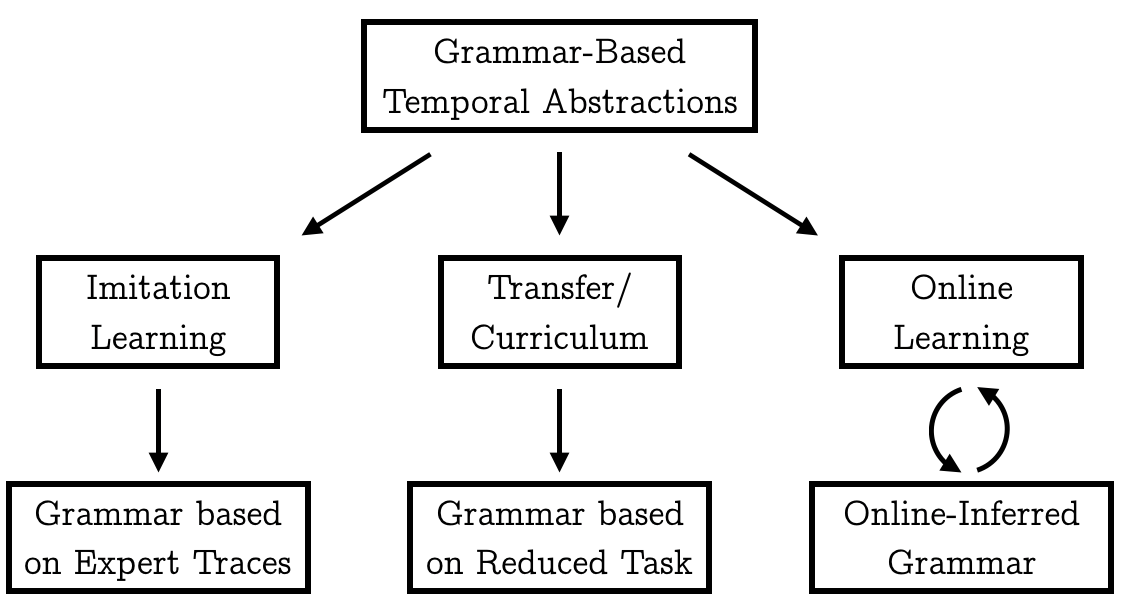
\includegraphics[width=\linewidth]{figures/concept_applications.png}
    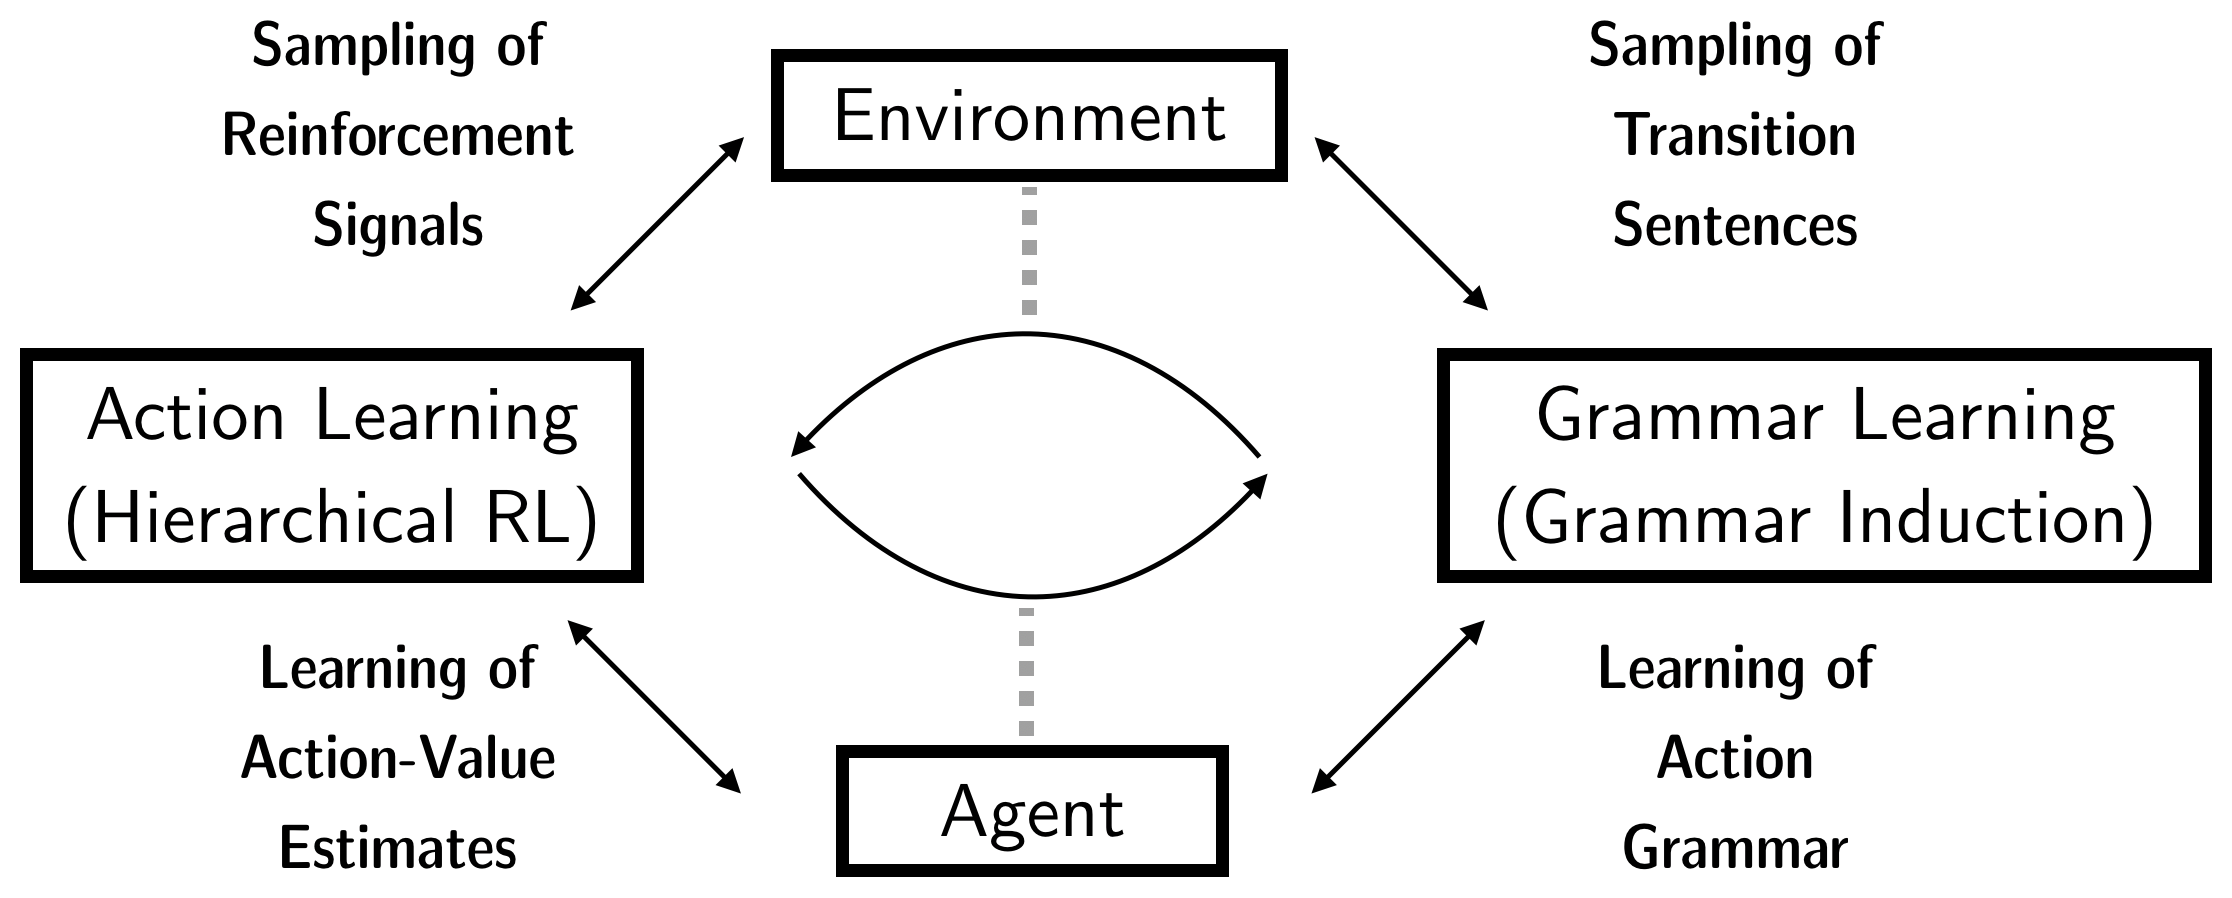
\includegraphics[width=\linewidth]{figures/concept_al_gl.png}
    \caption{Online-inferred action grammars alternation loop.}
    \label{fig:loop_ag}
\end{figure}

Our experiments highlight the usability of the action grammars framework for imitation learning and transfer learning given an expert policy rollout. Furthermore, we display strong results of an online version which iteratively refines grammar and value estimates. 

\section{Background}

\textbf{Temporal Abstractions.} 
%Learning a policy over temporally-extended actions allows the HRL agent to combat the uncertainty induced by single time-step decision making. The agent overcomes exploration problems, by restricting their decision process in a syntactically meaningful way.
SMDPs extend Markov Decision Process to incorporate not only reward and transition uncertainty but also time uncertainty. The time between individual decisions is modeled as a random variable, $\tau \in \mathbb{Z}_{++}$. It is characterized by the joint likelihood of transitioning from state $s \in \mathcal{S}$ into state $s'$ in $\tau$ time steps given action $m$ was pursued, $P(s', \tau| s, m)$. Thereby, SMDPs allow one to elegantly model the execution of actions which extend over multiple time-steps. A macro-action, $m \in \mathcal{M}$ specifies the sequential and deterministic execution of multiple ($\tau_m$) primitive actions. Let $r_{\tau_m} = \sum_{i=1}^{\tau_m} \gamma^{i-1} r_{t+i}$ denote the accumulated and discounted reward for executing a macro. Value estimates can then be updated using SMDP-Q-Learning \cite{Parr_1998a} in a model-free value-based manner:
$$Q(s, m)_{k+1} = (1-\alpha) Q(s, m)_k + \alpha \left( r_{\tau_m} + \gamma^{\tau_m} \max_{m' \in \mathcal{M}} Q(s', m')_k \right)$$  

In order to increase sample efficiency one can perform intra-macro updates for each state transition tuple $\{<s,a,r,s'>\}_{\tau_m}$ within the macro execution.
The DQN \cite{Mnih_2013, Mnih_2015} objective can easily be adapted:
$$L(\theta) := \mathbb{E} [(r_{\tau_m} + \gamma^{\tau_m} \max_{m' \in \mathcal{A} \cup \mathcal{M}} Q(s',m';\theta^-) - Q(s,m; \theta))^2] $$

The expectation is approximated by Monte Carlo samples from the macro experience buffer $\{s,m,r_{\tau_m},s', \tau\} \sim D_{\tau_m}$.

\textbf{Context-Free Grammars.} Given a start symbol $S$, a formal grammar $(\Sigma, \mathbb{N}, S, \mathcal{P})$ produces an output of strings. Production rules $\mathcal{P}$ map a set of non-terminal vocabulary $\mathbb{N}$ either to another non-terminal or terminal string within the terminal vocabulary $\Sigma$.
A context-free grammar (CFG) \cite{Chomsky_1959a} is such that production rules either map from one-to-one, one-to-none or one-to-many. A context-free grammar that is non-branching and loop-free is called a straight-line grammar. The process of inferring a grammar for a language that is consistent with a given sample of sentences is called grammar induction. Solutions to the smallest grammar problem \cite{Charikar_2005} attempt to infer the smallest CFG which compresses a string generated by a straight-line grammar. This problem is NP-hard \cite{Charikar_2005} and two greedy approximations are provided by Sequitur \cite{Manning_1997} and G-Lexis \cite{Siyari_2016b}.
Given a single sentence of the language, Sequitur sequentially reads in all symbols and collects repeating subsequences of symbols into a production rule. There while, the final encoded string is only allowed to have unique bigrams and production rules must be used more than once in the derivation of the string.
In order to overcome Sequitur's problem of noise overfitting, $k$-Sequitur \cite{Stout_2018} has been proposed. Instead of replacing a bigram with a rule if the bigram occurs twice, it has to occur at least $k$ times. As $k$ increases the discovered CFG grammar becomes less sensitive to overfitting noise and the resulting grammar is more parsimonious in terms of inferred production rules. 
%Lexis \cite{Siyari_2016b} provides an optimization-based alternative which iteratively constructs a directed acyclic graph (DAG). Starting from a trivial graph which connects a set of target sentences with the set of elements in the terminal vocabulary, the Lexis-DAG is constructed by adding intermediate nodes. Again, this problem by itself is NP-hard. G-Lexis, the greedy algorithmic implementation, searches for substrings that will lead to a maximal reduction in the cost, when added as new intermediate node.

\section{Context-Free Action Grammars}

 Action sequences as well as communication by the means of words both convey meaning and are goal-directed. Both consist of hierarchical structures and are conditioned by the environment in which they are uttered in. 
Many optimal policies $\pi^\star$ require a hierarchy of subgoal achievements which increase in sequential difficulty.
A trajectory obtained from traversing the current policy $\pi$ is viewed as a sample from the language generated by the grammar $L(\pi|E)$. Let the terminal vocabulary $\Sigma$ to consist of the primitive action space $\mathcal{A}$, hence $\Sigma = \mathcal{A}$. We denote  $\vartheta^i \sim L(\pi|E)$ for $i = 1, \dots N_g$ trajectories. Given a set of trajectories a CFG estimate $\hat{G}$ can be inferred and resulting production rules can be transformed into macro-actions by recursive flattening. The action space of the HRL agent is then augmented such that $\mathcal{A}^{\hat{G}} = \mathcal{A} \cup \mathcal{M}^{\hat{G}}$. Depending on the grammar compressed traces, one can construct several semantically-augmented action spaces:

\textbf{Expert \& Transfer Grammars.} If the traces $\vartheta^i$ are sampled from the language $L(\pi^\star|E)$ generated by the optimal policy, the agent can use the resulting grammar and flattened macros in an imitation learning setting. Furthermore, an agent faced with learning a sequence of tasks with increasing difficulty can make use of the optimal grammar of the previous task. Thereby, skills which are universal to all tasks do not have to be re-learned at every stage. 

  \begin{figure}
    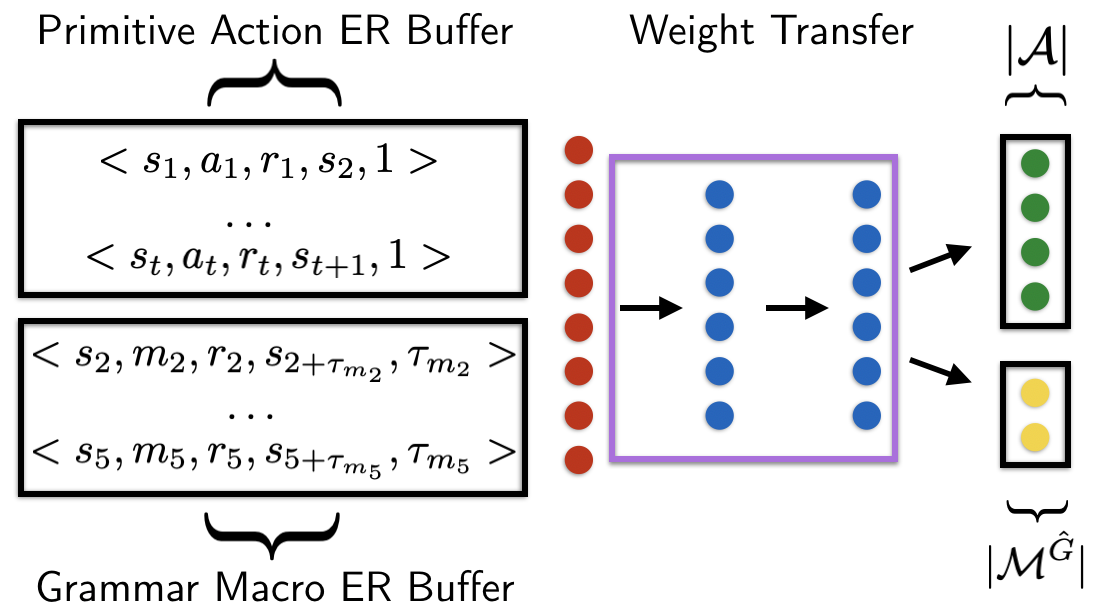
\includegraphics[width=\linewidth]{figures/ag_dqn_buffer}
    \caption{Grammar Transfer DQN with adaptive output head.}
  \label{fig:online_ag_dqn}
  \end{figure}
  

\textbf{Online Inferred Grammars.} Another approach is to alternate between grammar learning based on rollouts and action value refinements. If the episode successfully terminated, the grammar inference process identifies repeating patterns that led to successful goal achieving experiences.
In order to approximately preserve value estimates, we make use of transfer learning between grammar updates. The DQN architecture is altered as follows (see figure \ref{fig:online_ag_dqn}): In order to accommodate the variable set of grammar-inferred skills the size of the DQN output layer has to be updated after every grammar learning step yielding new macro-actions. By transferring the value-relevant features between action space augmentation, the agent can utilize the previously learned value characteristics. The weights of the final are then be relearned during the value learning. It is necessary to maintain a separate experience buffer system in order to store transition tuples specific to inactive previously inferred macro actions.  
Finally, we highlight the importance of adapting the hyperparameters of the grammar inference algorithm. The length of the sampled trace is going to increase or decrease over the course of the learning procedure. Hence, regularization parameter of the $k$-Sequitur grammar inference algorithm has to be changed accordingly.

\section{Experiments}

The goal of the experimental section of this work is to answer the following questions: (1) Does a grammar learned on optimal policy traces allow for rapid imitation learning? (2) Can CFG grammars be used in order to enhance curriculum as well as transfer learning? (3) Is online grammar inference and action space adaptation able to structure the exploration process of the HRL agent?
In order to illustrate our results we choose the $N$-disk Towers of Hanoi (ToH) environment (see figure \ref{fig:hanoi}).
%The general game setting for $N$ disks is as follows: In every episode of the game the agent is initialized in the tuple $(1)_{i=1}^N$. At each point in (discrete) time the agent transitions between states with the help of the following moves:  $\mathcal{A} = \{a:(1,2); b:(1,3); c:(2,1); d:(2,3); e:(3,1); f:(3,2)\}$.
The agent maximizes their expected cumulative discounted reward by reaching the final state $(3)_{i=1}^N$ as quickly as possible. The problem is formulated as a sparse long-term credit assignment problematic. The size of the state space, on the other hand, grows exponentially, $|S| = 3^N$ (all possible allowed orderings), and the optimal number of moves to solve this game is given by $2^N - 1$. Identifying this underlying hierarchical principle and generalizing between different environments requires the agent to correctly identify their state in the underlying hierarchical action parse tree.

\begin{figure}
    \centering
    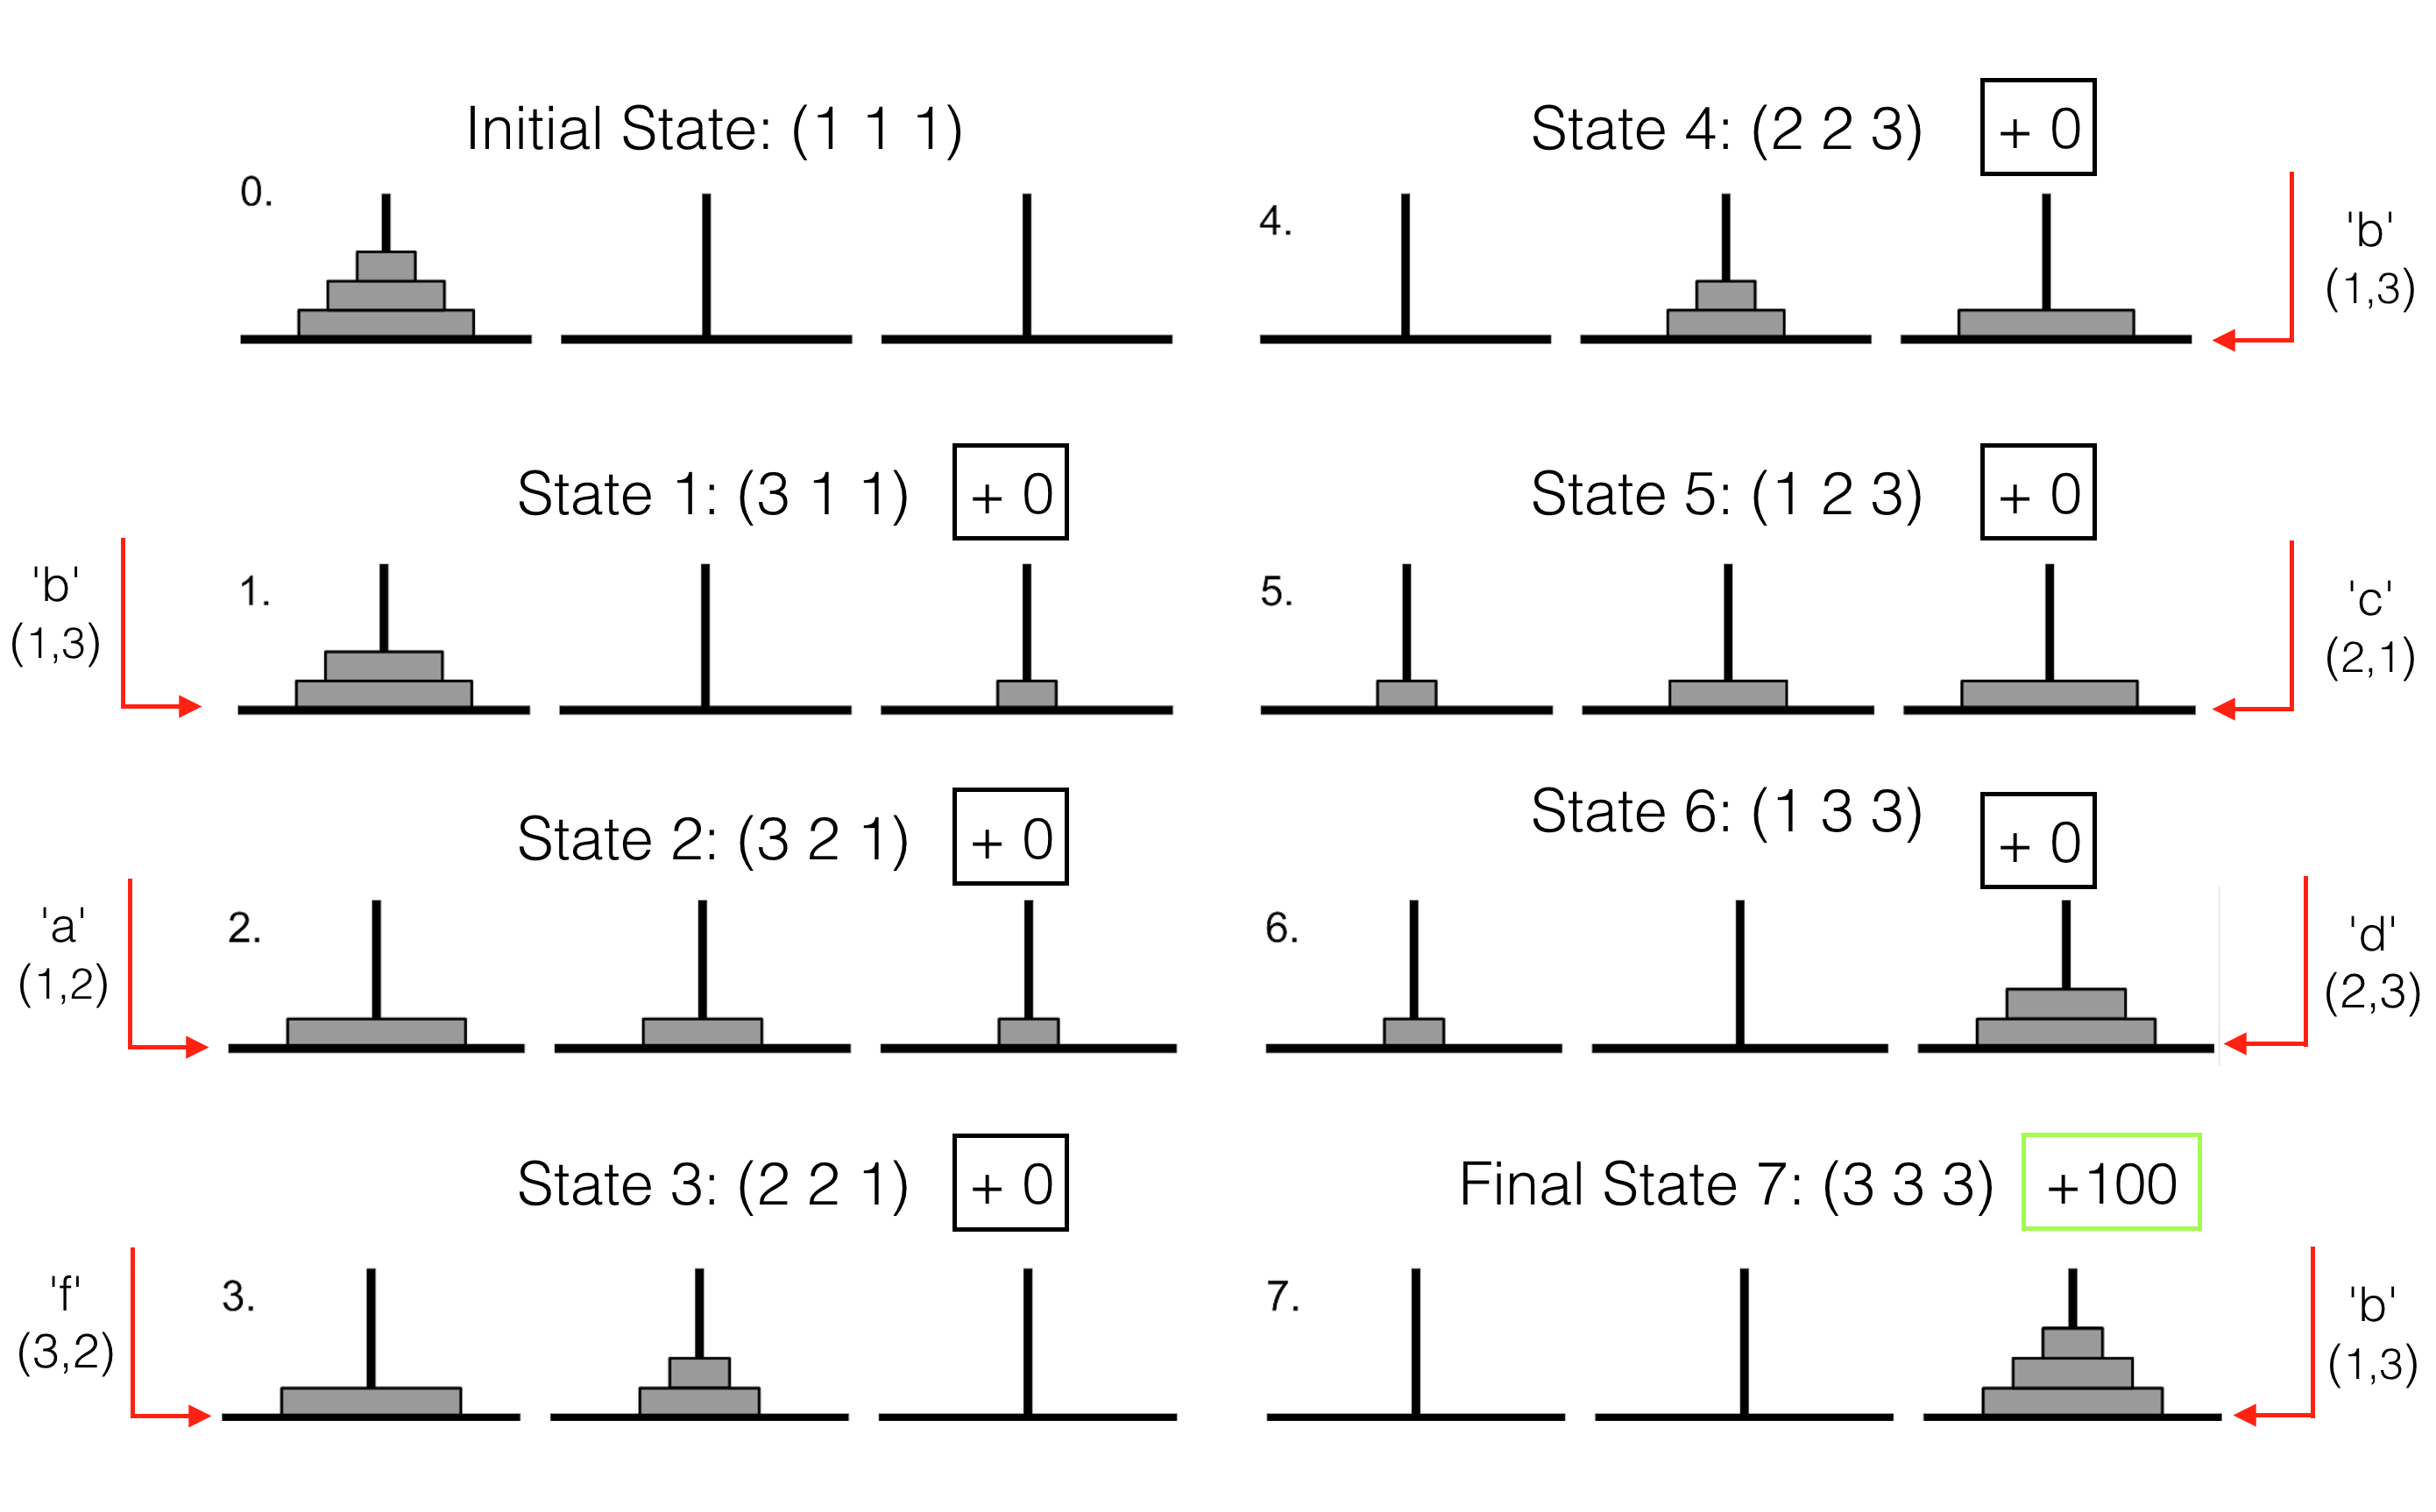
\includegraphics[width=\linewidth]{figures/hanoi_problem.png}
    \caption{RL Formulation of the ToH Problem}
    \label{fig:hanoi}
 \end{figure}
 

  \begin{table}
    \centering
    \begin{tabular}{c | c c |} % centered columns (4 columns)
\hline\hline %inserts double horizontal lines
 \multicolumn{3}{c}{Trace ($\vartheta$): bafbcdbafec} \\
 \multicolumn{3}{c}{fbafbcdbcfecdbafbcdb}\\
\hline
\hline
 $\vartheta^{enc}$ & \multicolumn{2}{c}{BCDfBEfDdBb} \\
 $\frac{|\vartheta^{enc}|}{|\vartheta|}$ & \multicolumn{2}{c}{0.355}\\
 %$\frac{\mathcal{H}(\vartheta^{enc})}{\mathcal{H}(\vartheta)}$ & \multicolumn{2}{c}{1.0702} & \multicolumn{2}{c}{1.3613}\\
\hline \hline
$\mathbb{N}$ & PR & $\mathcal{M}^{2-Seq}$ \\ % inserts
\hline % inserts single horizontal line
B & CEd & bafbcd \\
C & - & baf \\
D & - & ec\\
E & - & bc\\ 
\hline %inserts single line
\end{tabular}
      \caption{2-Sequitur ToH (5 disks) Grammar-Macros}
      \label{table:optimal_grammar}
\end{table}
  

%-----------------------------------
\textbf{Learning with Expert \& Transfer Grammars.} Given action sequences of an expert the HRL agent can infer a set of grammar macros and augment their action space. Table \ref{table:optimal_grammar} displays the grammar macros inferred from a trace of the optimal policy using the 2-Sequitur as well as the G-Lexis algorithm. The flattened production rule $B \to CEd \to bafbcd$ captures the recursive nature learned by the grammar. $C \to baf$ moves two disks on the auxiliary pole, while $E \to bc$ moves a third disk from source to target pole and one disk back onto the source pole. We can then augment the action space of the 5 disk agent in the following way:

$$\mathcal{A}^{\hat{G}} = \mathcal{A} \cup \mathcal{M}^{2-Seq} = \mathcal{A} \cup \{bafbcd, baf, ec, bc\}$$

%\begin{figure}[H]
%\minipage{0.33\textwidth}
%  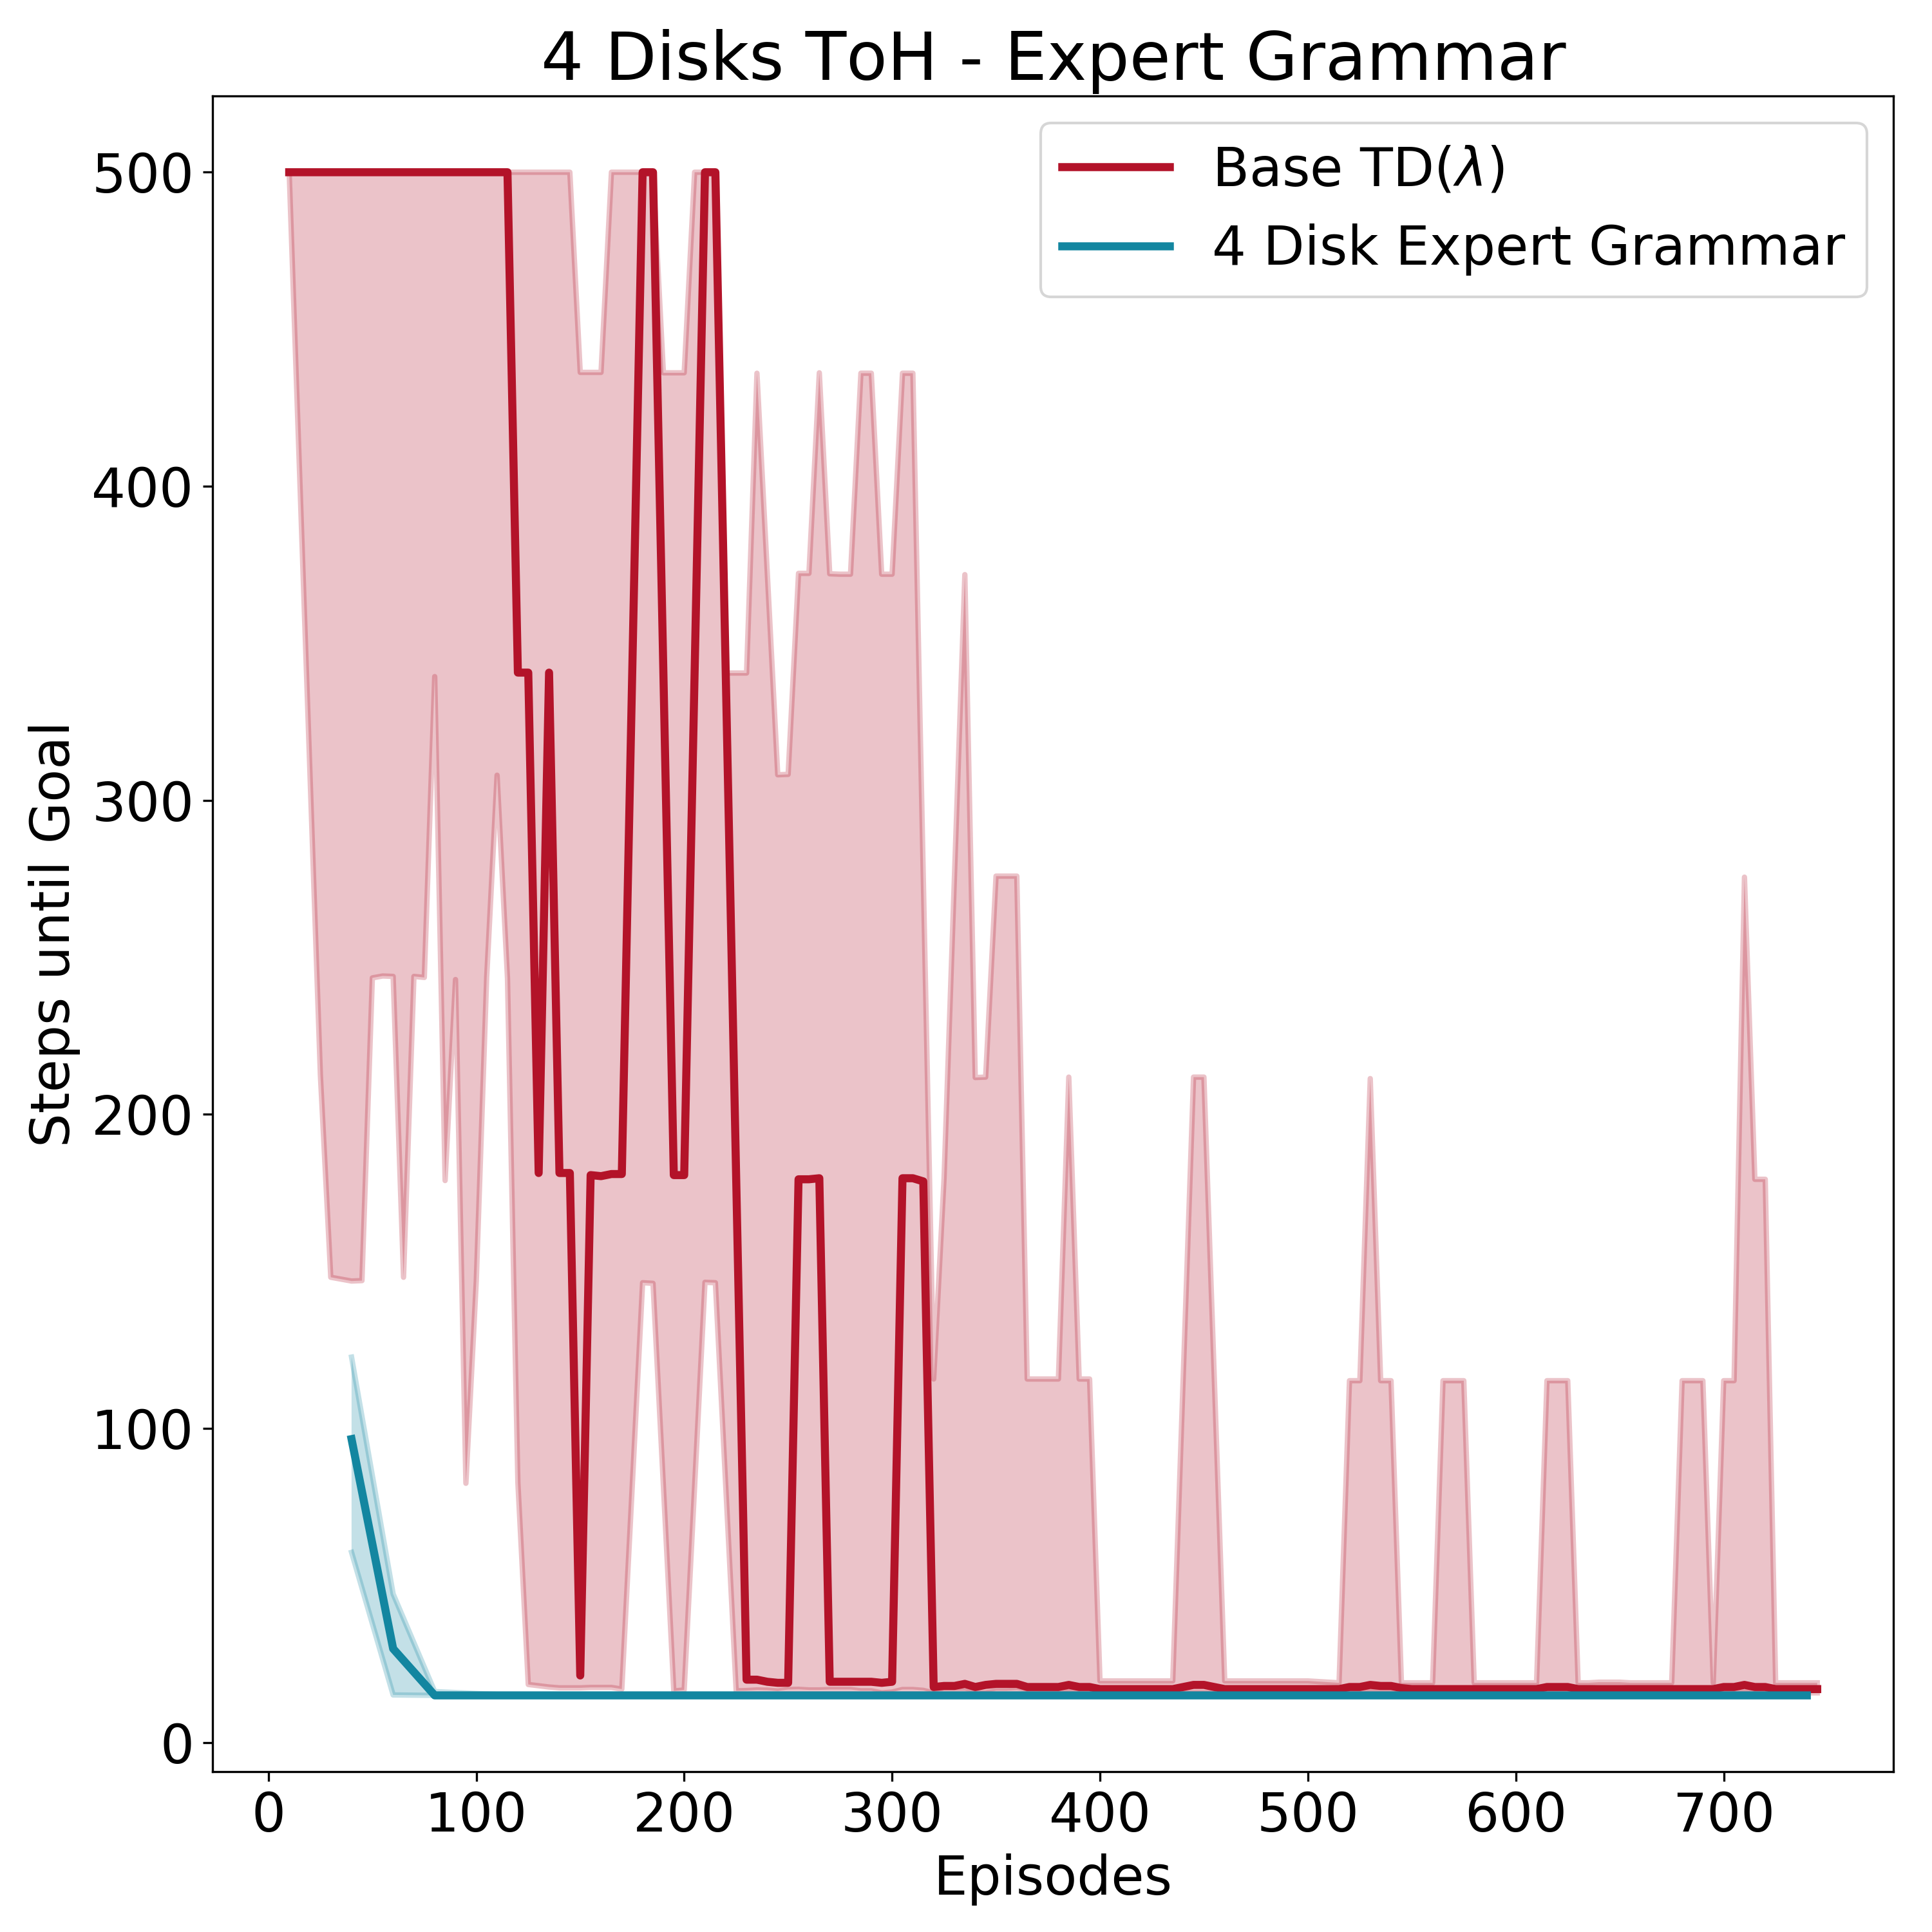
\includegraphics[width=\linewidth]{figures/4_disks_transfer_grammar}
%\endminipage\hfill
%\minipage{0.33\textwidth}
%  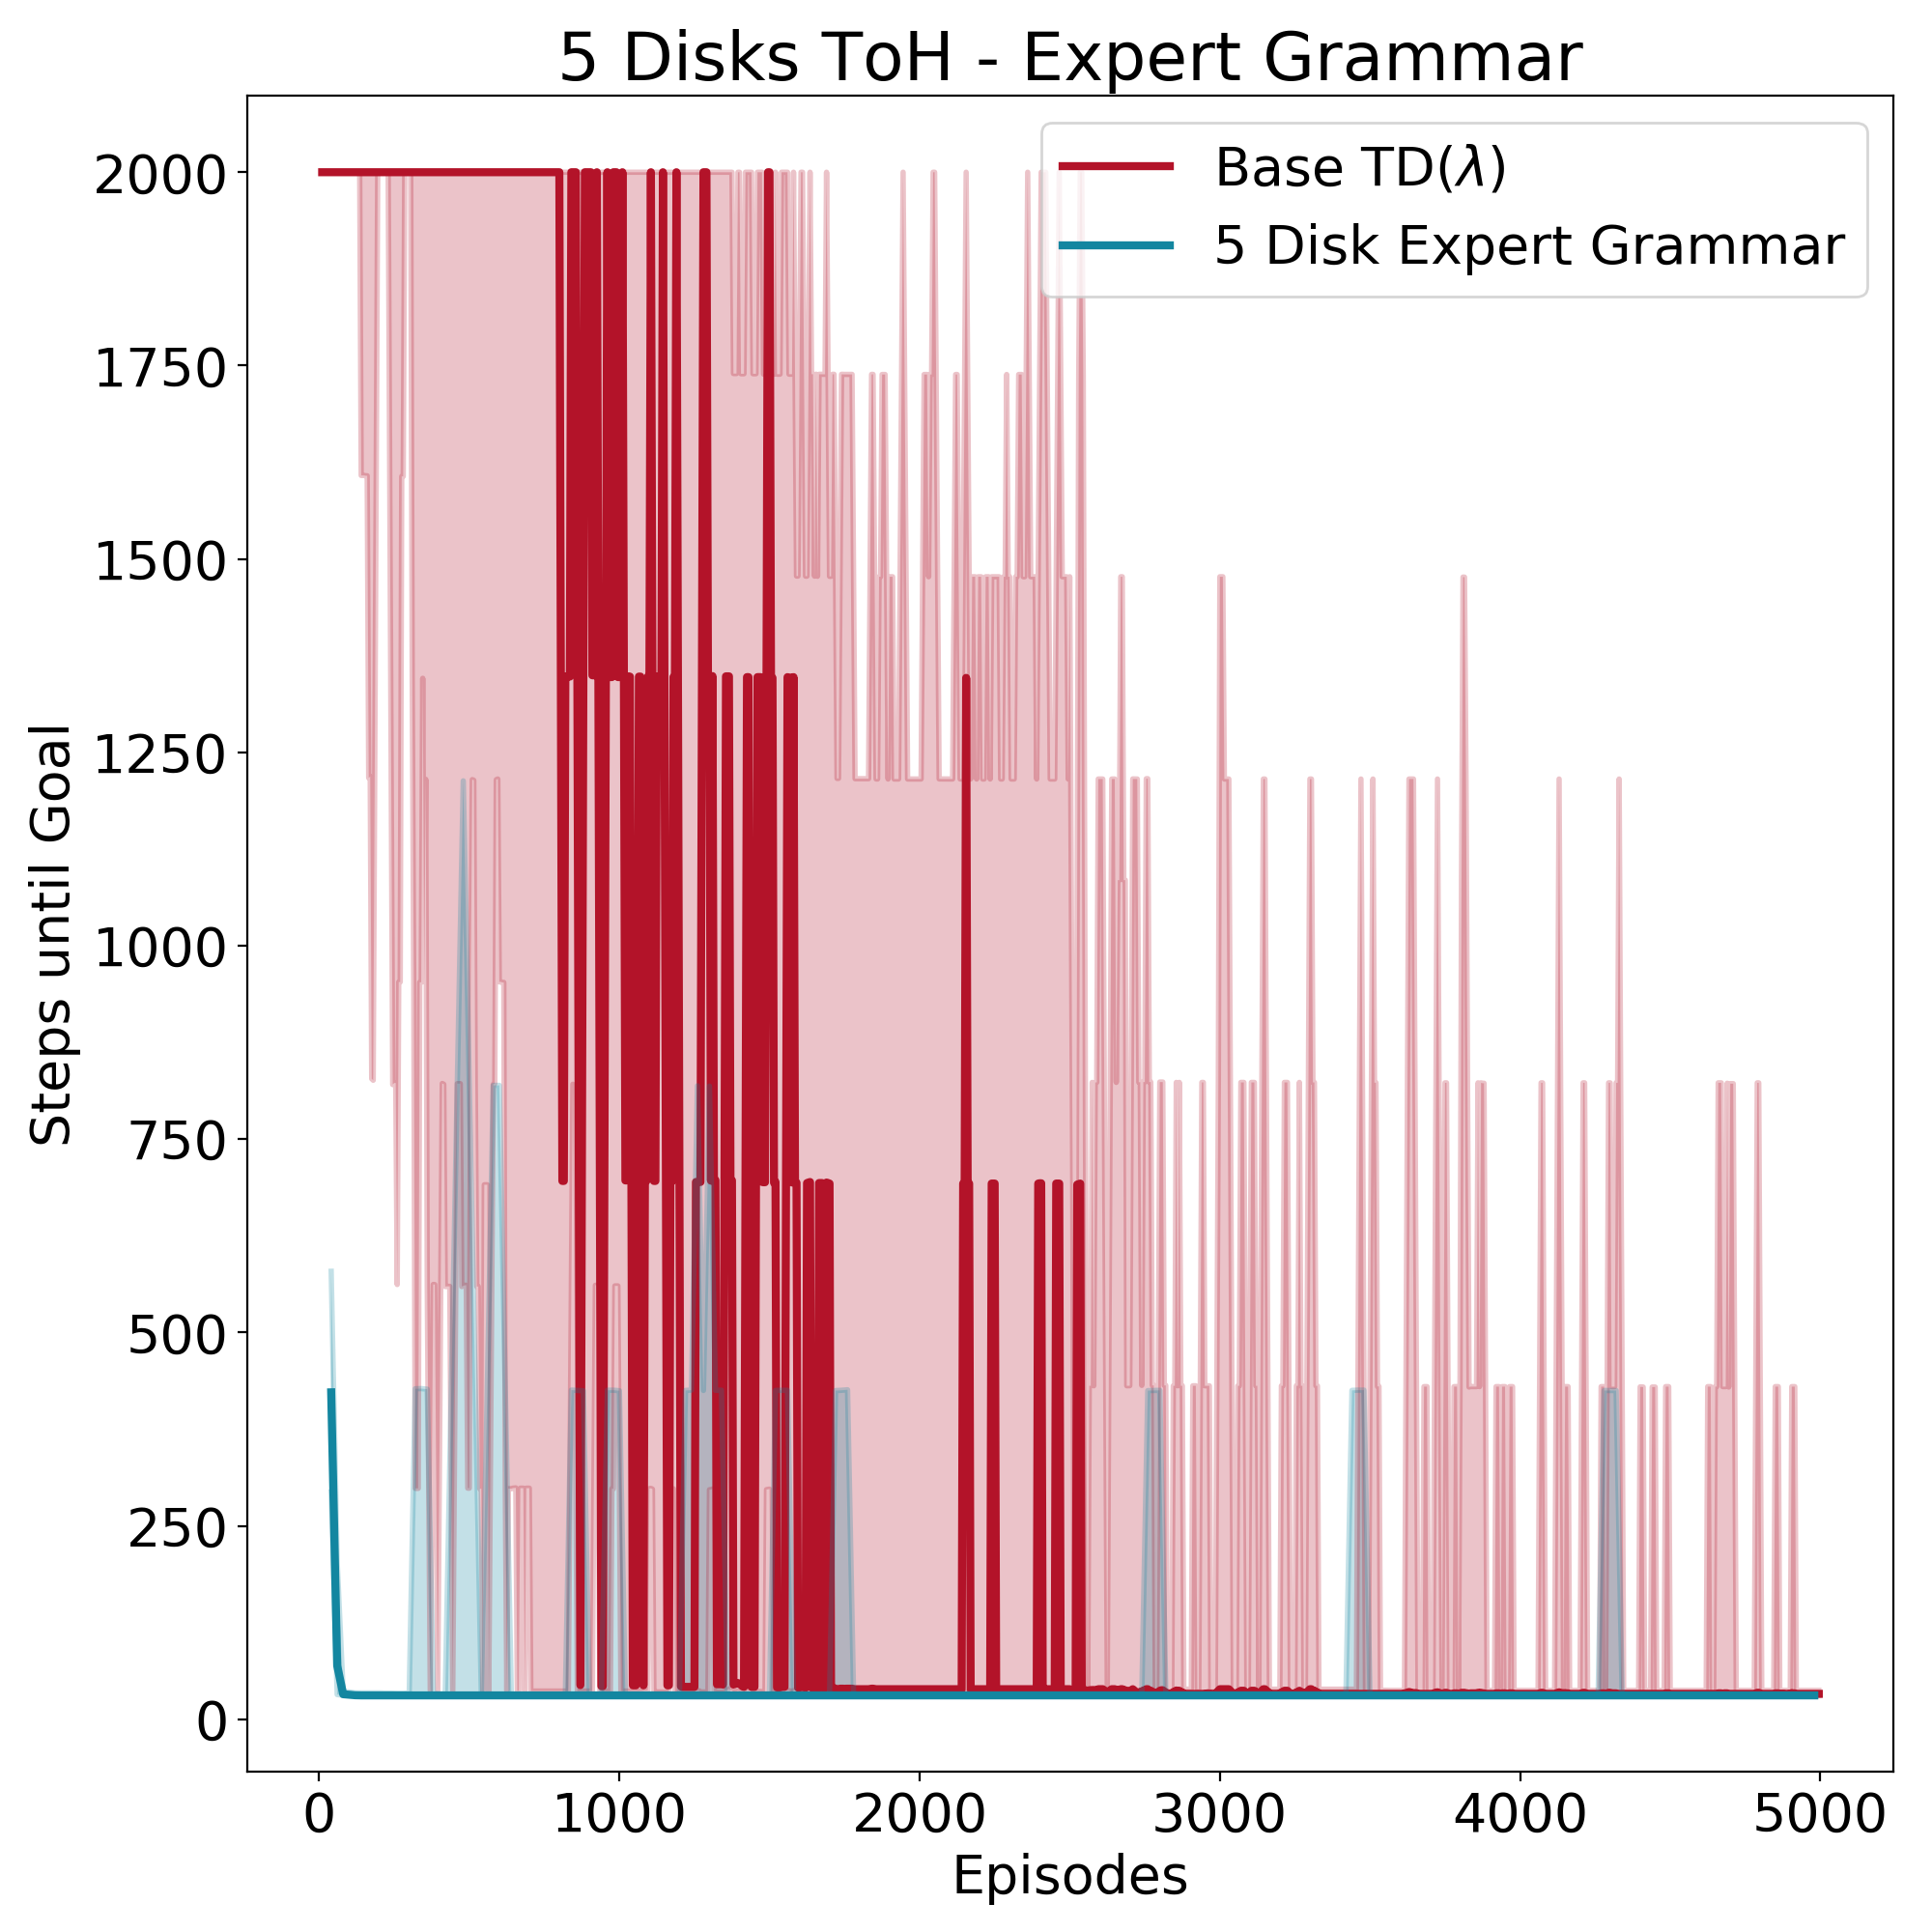
\includegraphics[width=\linewidth]{figures/5_disks_transfer_grammar}
%\endminipage\hfill
%\minipage{0.33\textwidth}%
%  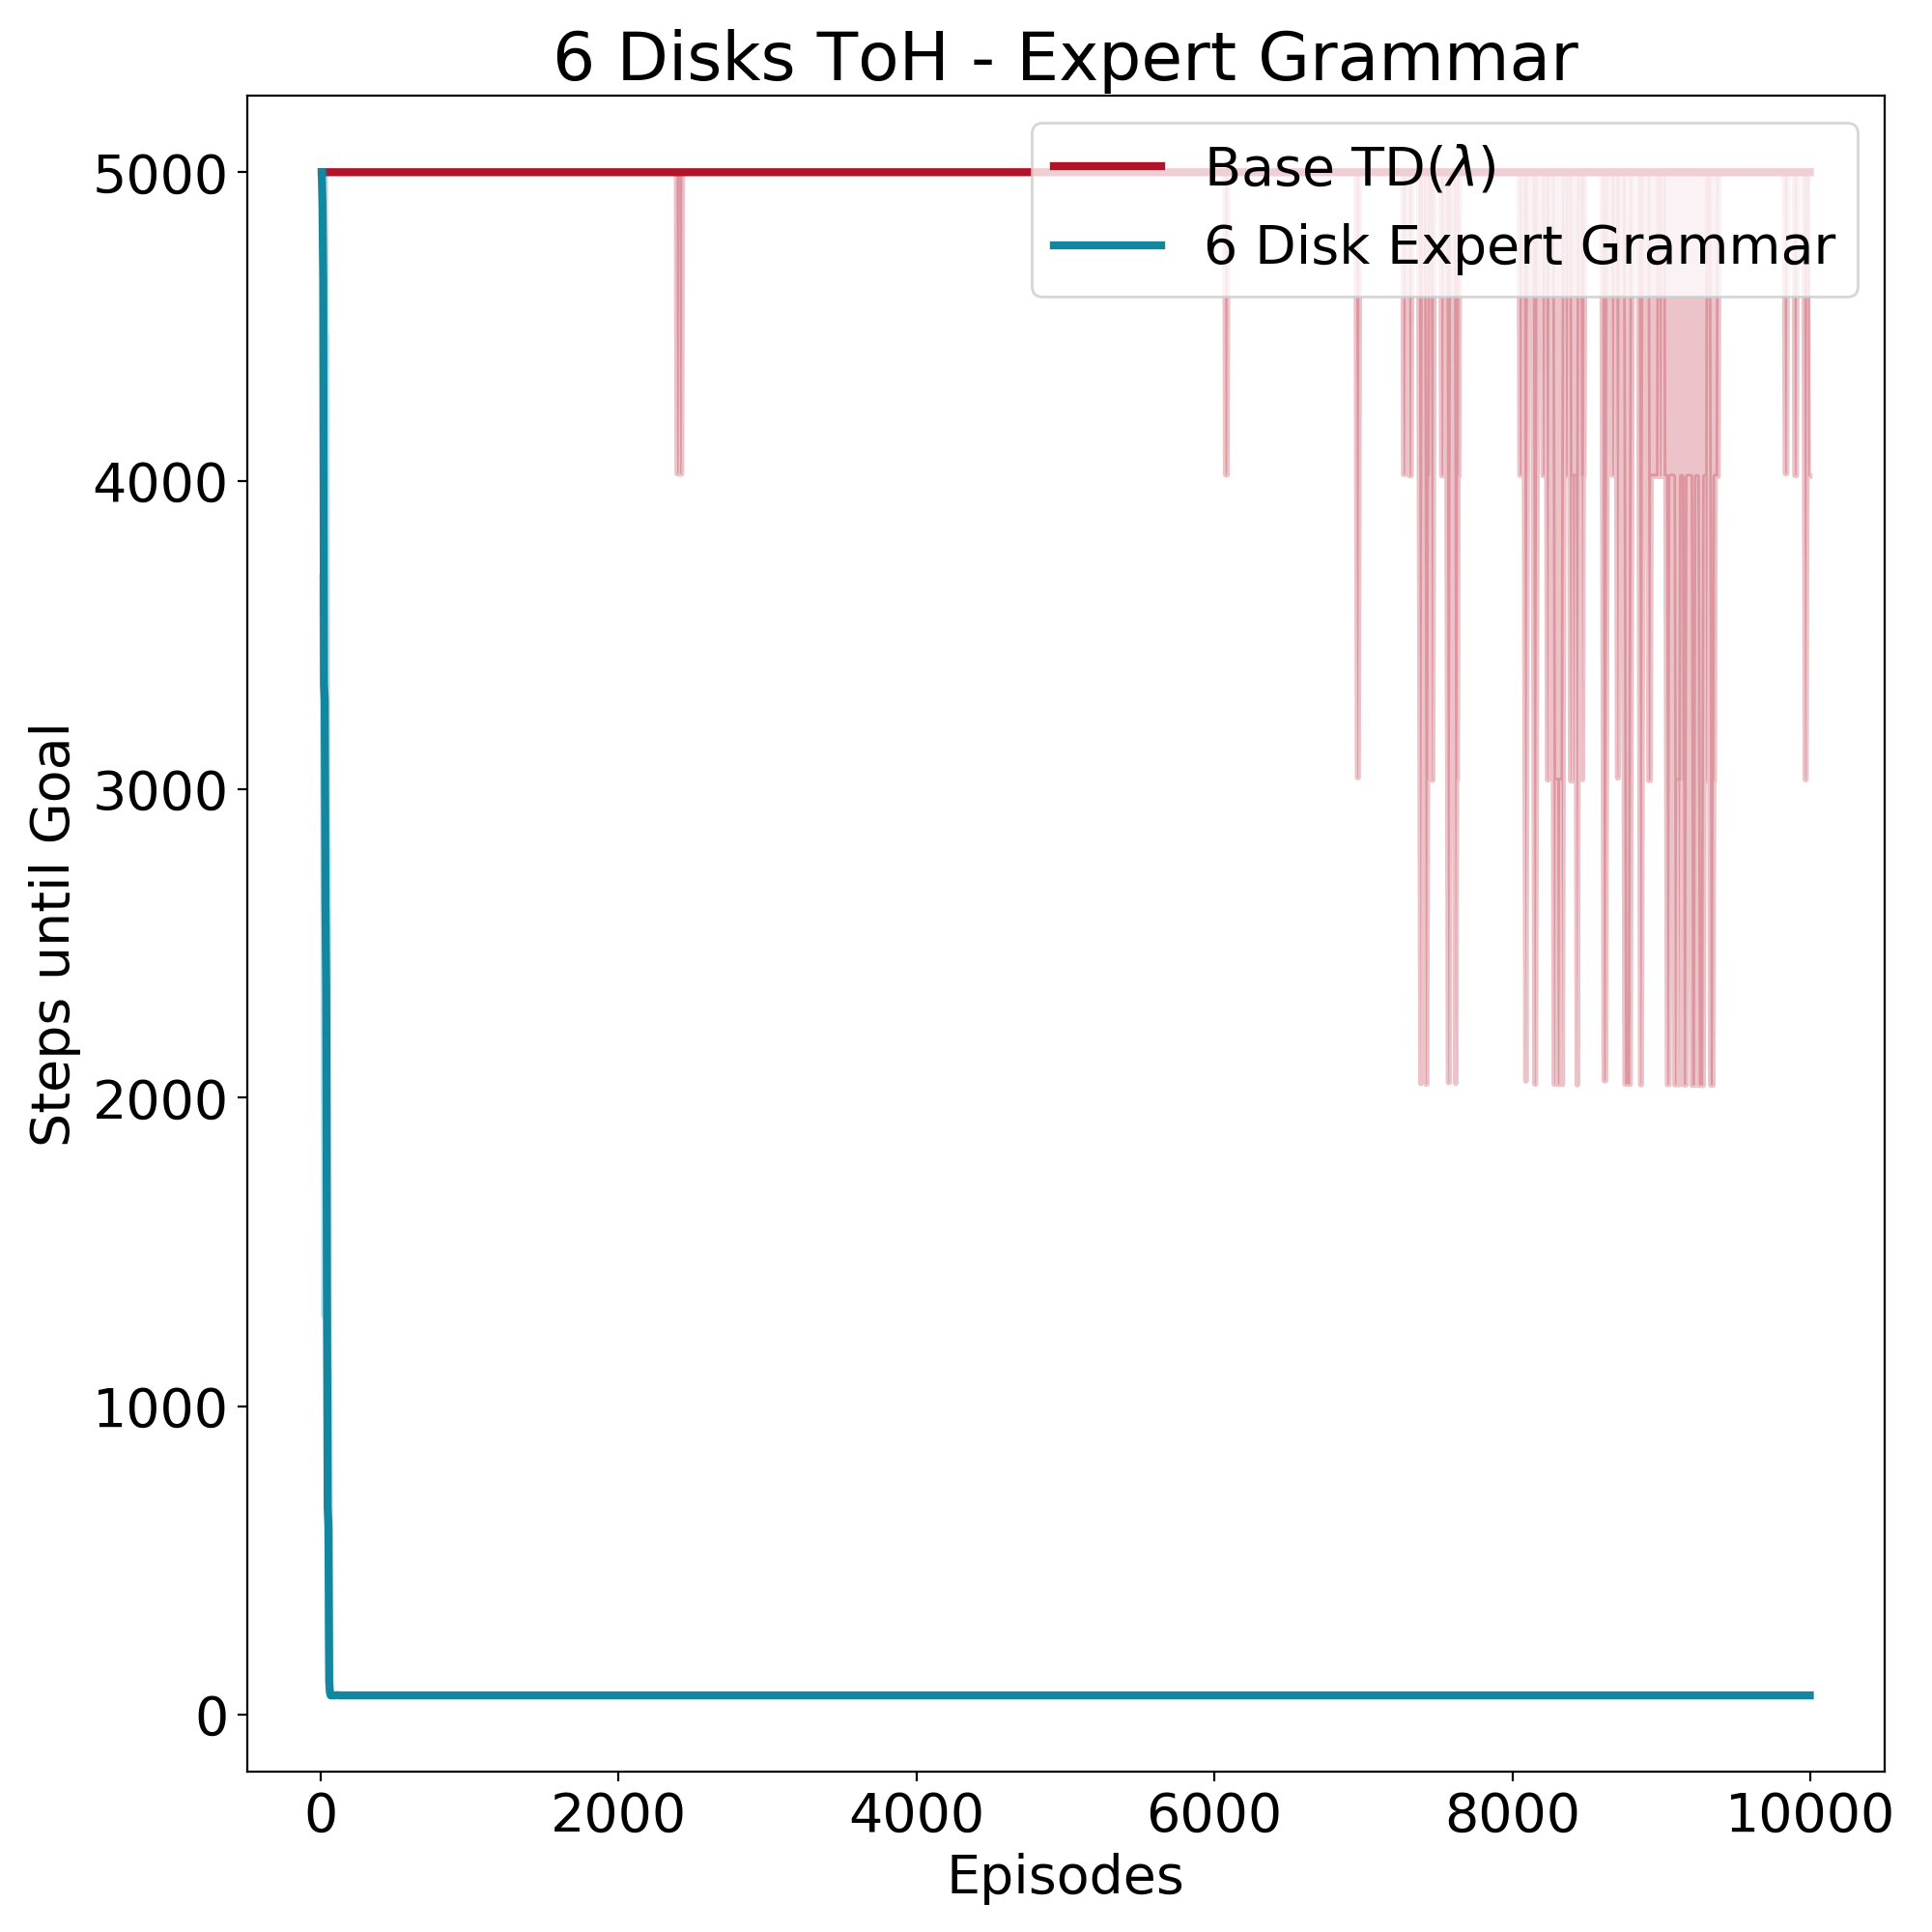
\includegraphics[width=\linewidth]{figures/6_disks_transfer_grammar}
%\endminipage
%\caption{Learning Results for SMDP-Q-Learning with Expert Grammar Macros for 4, 5 and 6 Disk Environment. Median, 10th percentile and 90th percentile reported over 5 runs.}
%\label{fig:expert_grammar}
%\end{figure}

Figure \ref{fig:expert_grammar} displays learning results for different SMDP-Q-Learning agents with macro-actions defined by the production rules inferred from a trace of the optimal policy. One can observe that the grammar macros greatly accelerate the learning progress of the agent. Furthermore, the variance of rollouts is greatly reduced due to increased robustness. Instead of using the optimal grammar macros for a specific environment, we are also interested in assessing how well the grammars learned for a more simplistic environment (i.e. $N-1$ disks).  


%\missingfigure[figwidth=\textwidth]{Learning Result for Transfer Grammar}
%
%\begin{figure}[H]
%\minipage{0.475\textwidth}
%  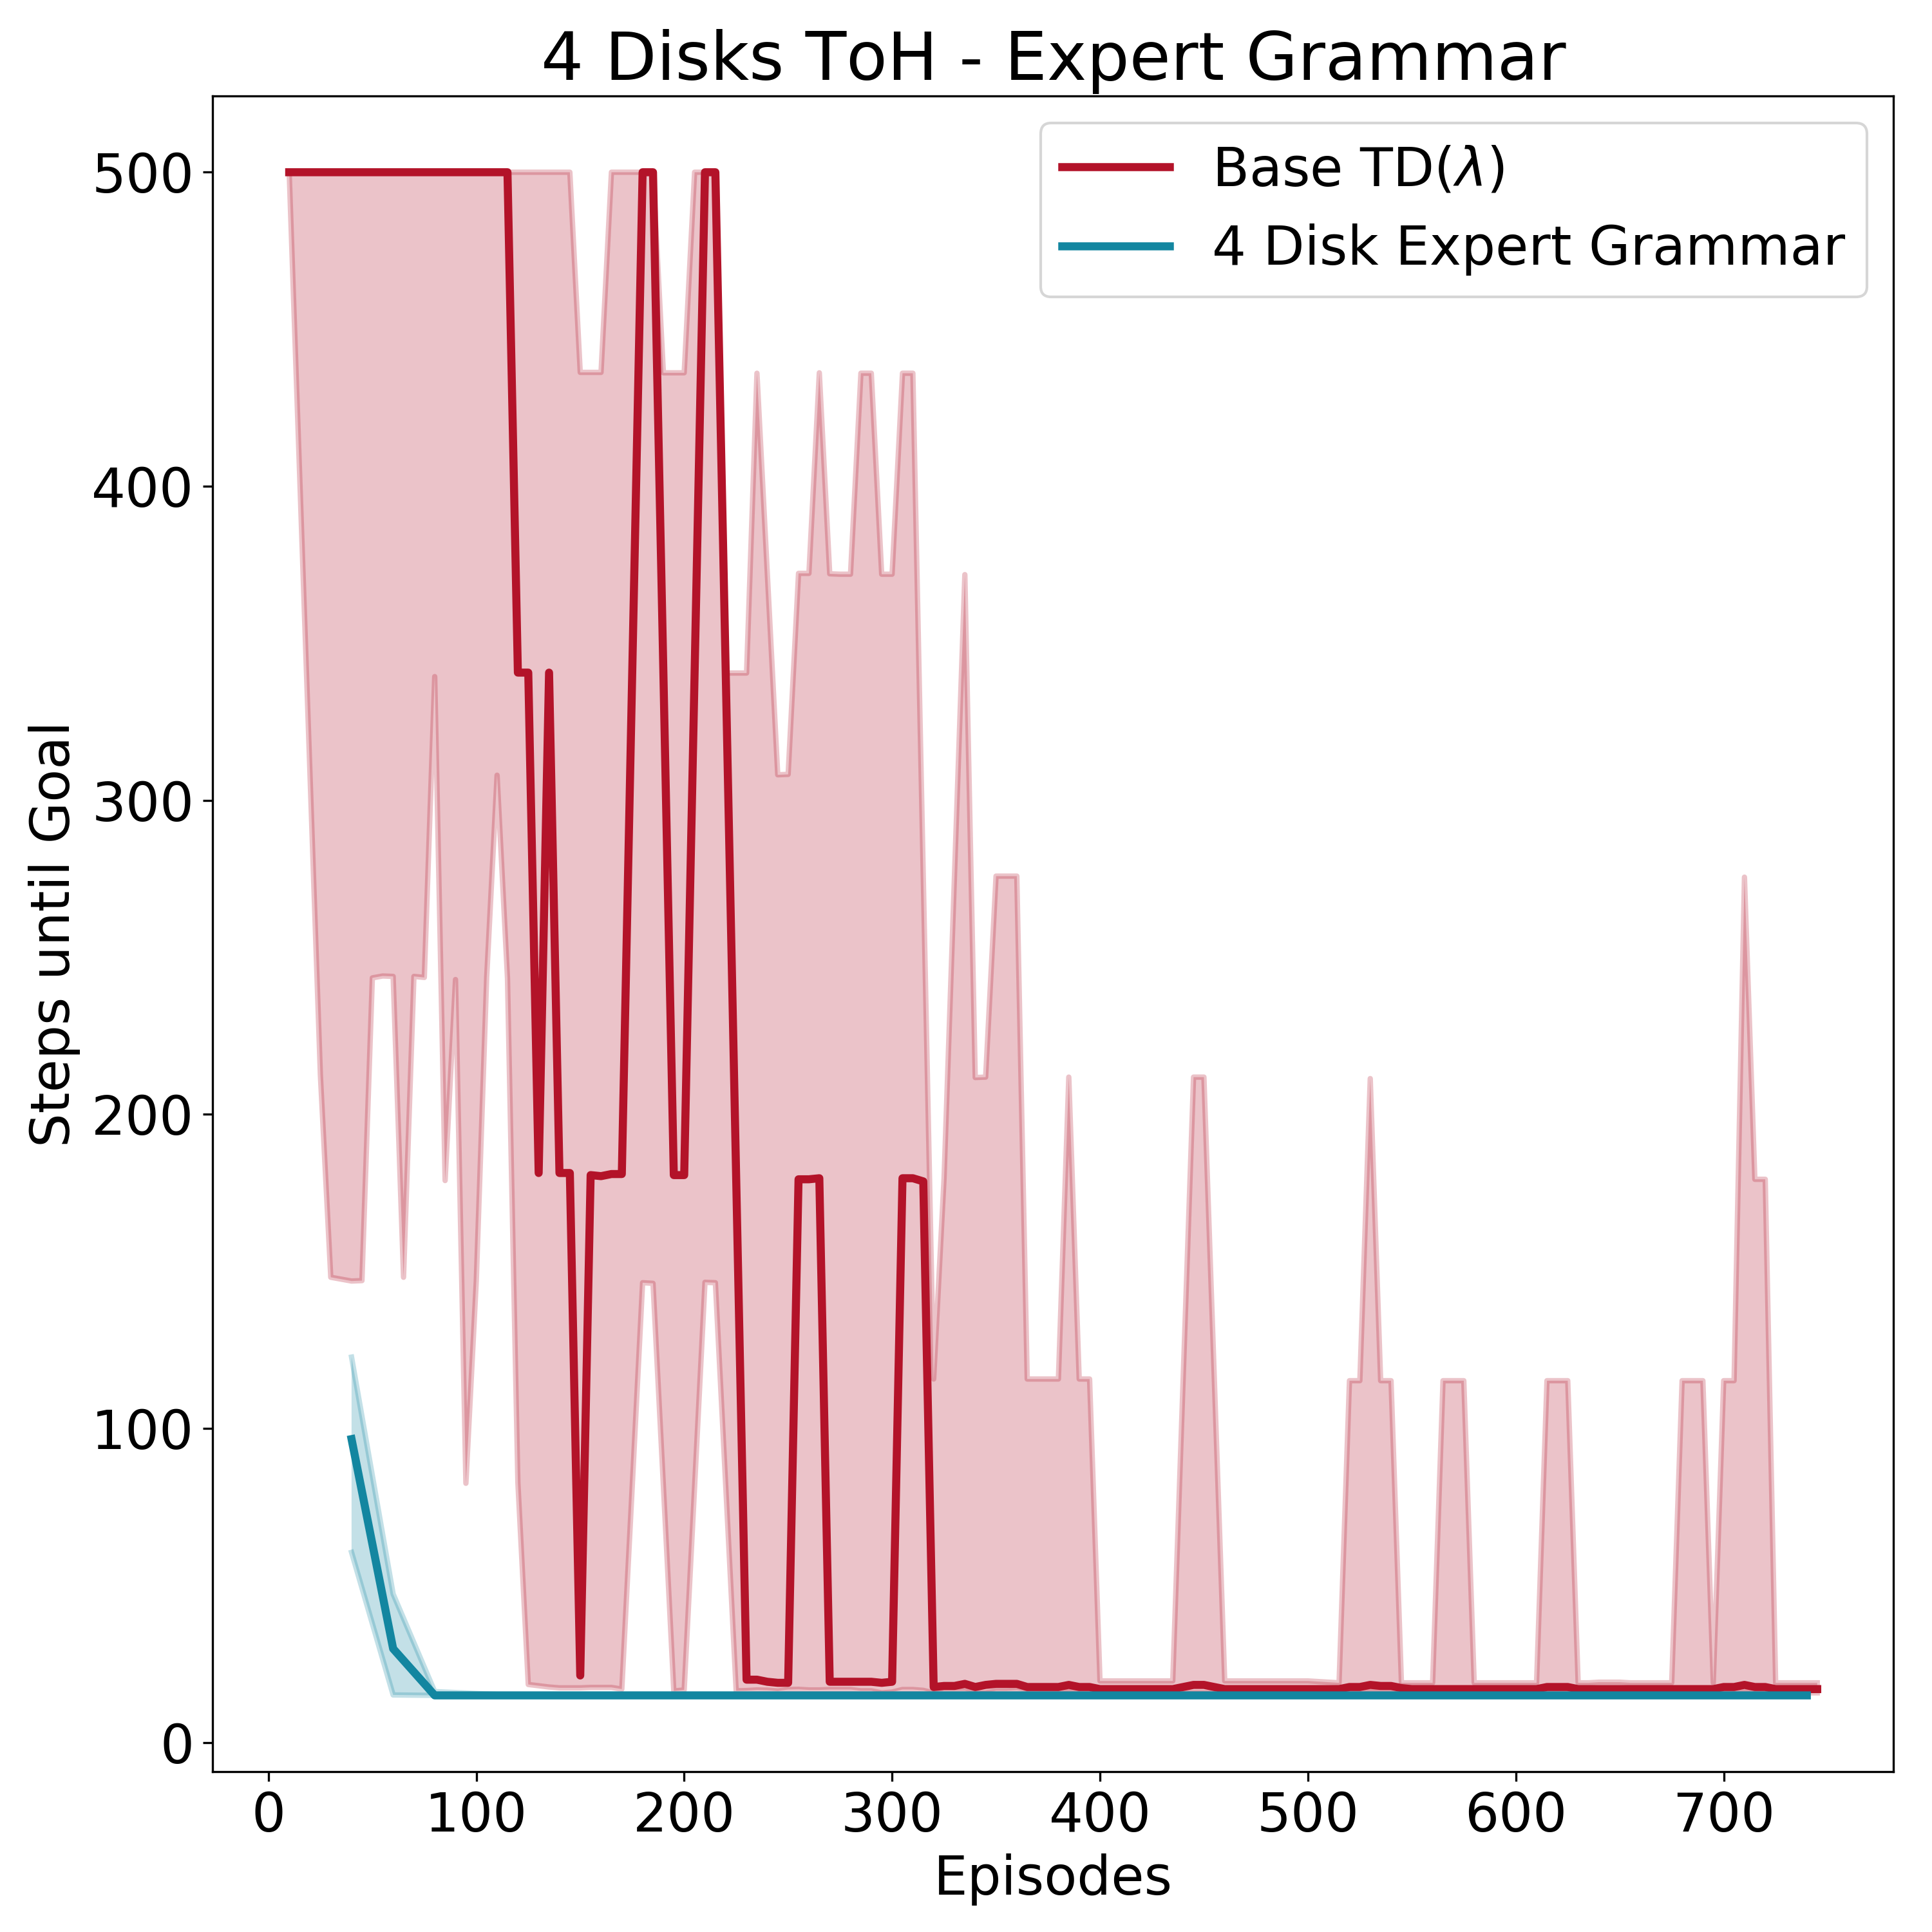
\includegraphics[width=\linewidth]{figures/4_disks_transfer_grammar}
%\endminipage\hfill
%\minipage{0.475\textwidth}
%  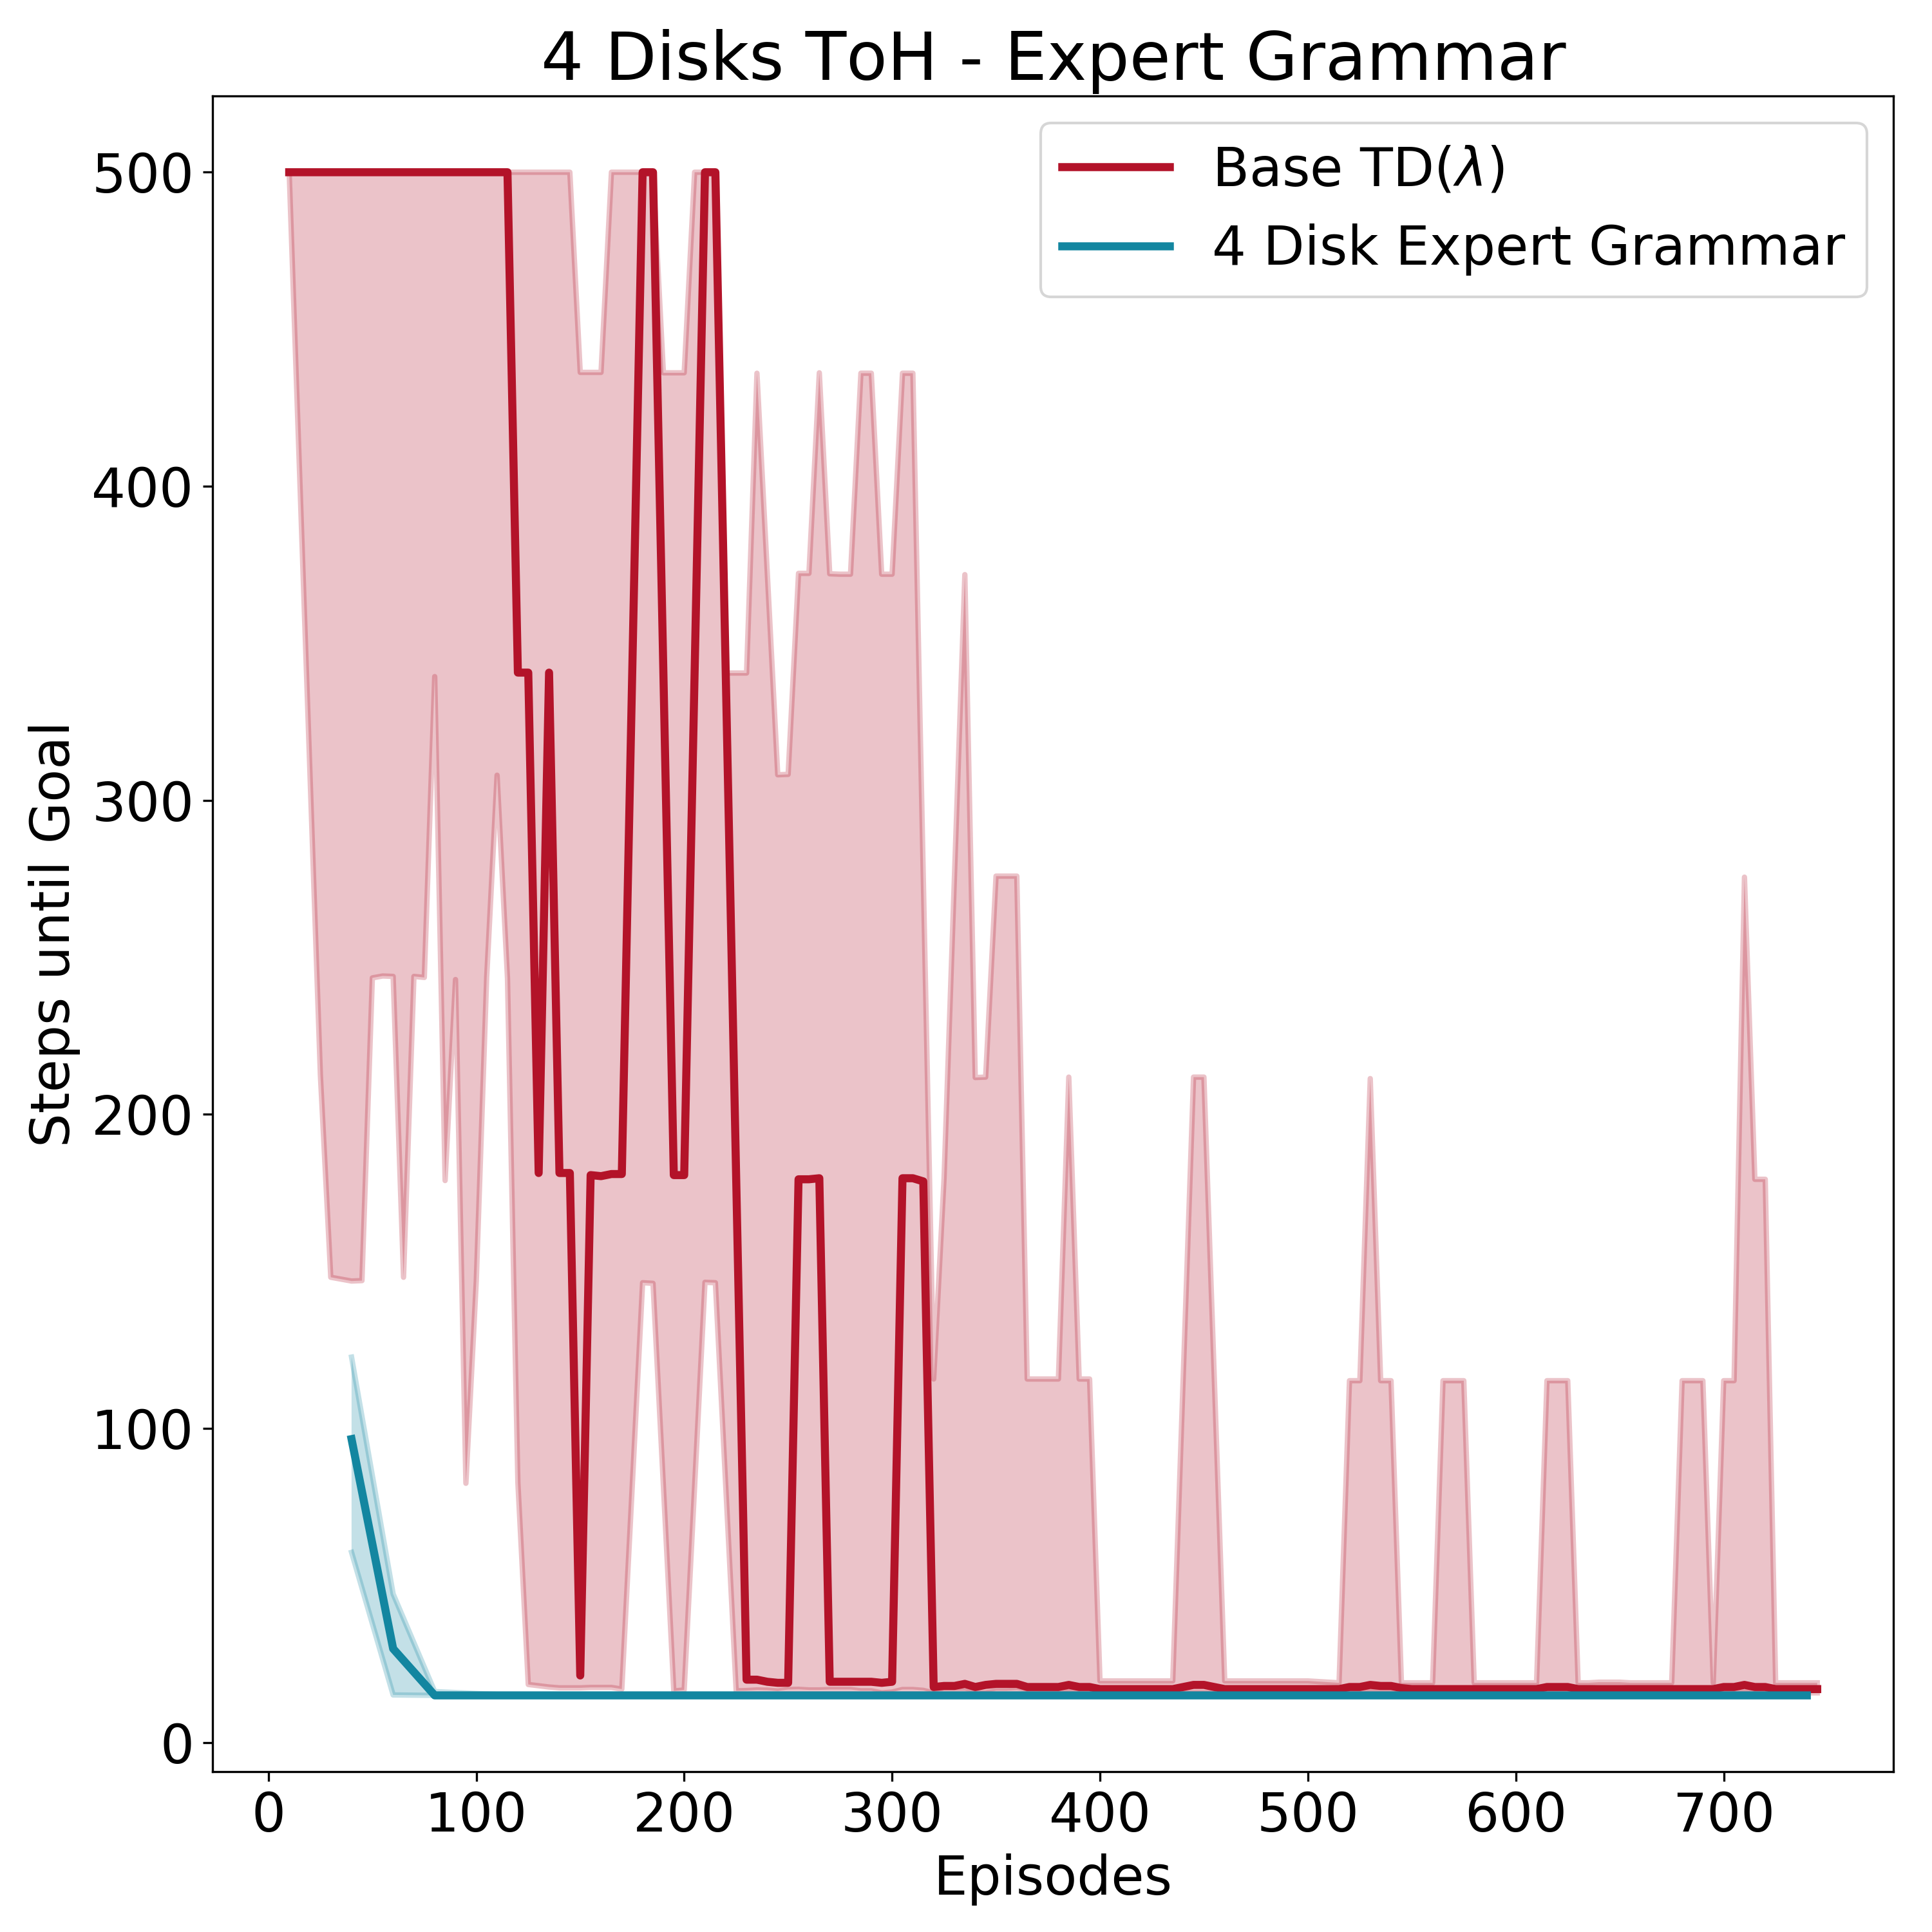
\includegraphics[width=\linewidth]{figures/4_disks_transfer_grammar}
%\endminipage\hfill
%\caption{Learning Results for SMDP-Q-Learning with Transfer Grammar Macros for 5 and 6 Disk Environment. Median, 10th percentile and 90th percentile reported over 5 runs.}
%\label{fig:transfer_grammar}
%\end{figure}


%-----------------------------------
\textbf{Learning with Online Inferred Grammars.}

%\missingfigure[figwidth=\textwidth]{Learning Result for Online Inferred Grammar}
%
%\rob{Add Grammar DQN experiments.}

\section{Conclusion}

Motivated by a parallelism between the hierarchical generating processes of language and motion, we have derived multiple algorithmic approaches which exploit powerful grammatical inference frameworks to identify temporally-extended actions.By sensibly defining temporally-extended actions and abstracting away unnecessary decision points, one is able to overcome the curse of dimensionality. 
In order to validate our proposed framework, we tested the approach on an imitation learning as well as an online RL task. Our contributions can be summarized as follows:
%
(1) The CFG approach to macro-actions extraction from flat production rules performs well in both imitation and transfer learning. The agent can easily generalize from the inferred hierarchical structure and is able to increase the action learning speed drastically.
%
(2) Alternating between grammar updates and learning action values is an effective way of both online learning of an optimal grammar as well as an optimal policy. The first grammar extraction and action space augmentation has the largest significant effect in the further learning procedure of the agent. 

%In future work we are interested in testing and extending our approach to physical and continuous (joint and velocity-bases state representations, e.g. MoJuCo) domains as well as model-based methods. Formal grammars are especially useful for languages with large terminal vocabulary. So far we have only experimented with discrete action spaces and single agents. \cite{Pastra_2012} note that social interactions of more than one agent can also be formulated within the notion of tool use. Hence, we are interested in possible applications to multi-agent RL  and testing the scalability of our approach to real-life domains.
%
%Furthermore, our approach has only attempted to merge grammatical inference with one HRL algorithm. There remain many other promising frameworks such as the Hierarchies of Abstract Machines (HAMs, \cite{Parr_1998a,Parr_1998b}). HAMs define a hierarchy over finite state machines. This could naturally lead itself to automated identification via Hierarchical Hidden Markov Models \cite{Fine_1998}.
%
%Future work also has to further analyze the development of the inferred grammar throughout the learning process. Edit distances such as the Levenshtein and Jaro-Winkler distance provide two measures of string similarity which might be used to efficiently monitor the development of the inferred flat productions compared with the optimal grammar.
%
Ultimately, we envision a form of dictionary of action which provides an expandable library of skills for Hierarchical Reinforcement Learning agents which act in diverse naturalistic environments. This could provide a mayor contribution to a key endeavor in general artificial intelligence: Life-long learning.

\newpage
\bibliographystyle{apacite}

\setlength{\bibleftmargin}{.125in}
\setlength{\bibindent}{-\bibleftmargin}

\bibliography{HRL}


\end{document}
